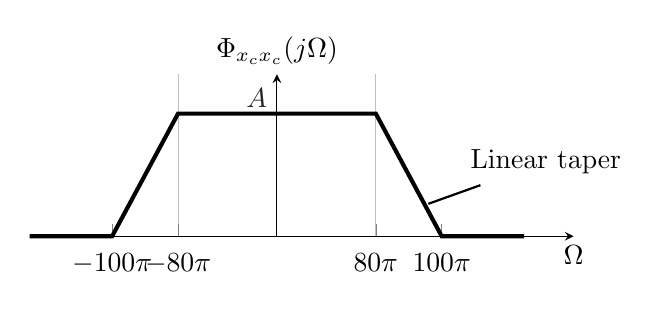
\begin{tikzpicture} 
\begin{axis}[
axis lines*=middle,
enlargelimits = upper, clip=false,
width=0.7\textwidth,
height=0.3\textwidth,
ymin=0,
ymax=1.2,
xmin=-15,
xmax=15,
axis line style={->,>=stealth},
xlabel={$\Omega$},
ylabel={$\Phi_{x_cx_c}(j\Omega)$},
yticklabel style = {yshift=0.2cm},
xticklabel style = {yshift=-0.1cm},
every axis x label/.style={
	at={(ticklabel* cs:1)},
	anchor=north,
},
every axis y label/.style={
	at={(ticklabel* cs:1)},
	anchor=south,
},
ytick=1,
yticklabels={$A$},
xtick={-10,  10},
xticklabels={$-100\pi$, $100\pi$},
extra x ticks={-6, 6}, extra x tick labels={ $-80\pi$, $80\pi$},
extra tick style={grid=major},
every outer y axis line/.append style={white!15!black},
every y tick label/.append style={font=\color{white!15!black}},
legend style={draw=white!15!black,fill=white,legend cell align=left}]

\addplot[black, line width=1.5pt] coordinates {(-15, 0) (-10, 0) (-6, 1) (6, 1) (10, 0) (15, 0)} node[->, pos=0.8, black, pin={[pin edge={black, thick}]30:{Linear taper}}, inner sep=0pt] {};
\end{axis}
\end{tikzpicture}